\documentclass[conference]{IEEEtran}

\usepackage{url}
\usepackage{graphicx}
\usepackage{caption}
\usepackage{subcaption}
\usepackage{hyperref}
\usepackage{url}
\usepackage{times}
\usepackage{balance}
\usepackage{xspace}
\usepackage{paralist}
\usepackage{color}
\usepackage{booktabs}
\usepackage[usenames,dvipsnames]{xcolor}
\usepackage{amssymb}

\clubpenalty = 10000
\widowpenalty = 10000
\displaywidowpenalty = 10000

\begin{document}

\newcommand{\ghtorrent}{ \textsc{ght}orrent\xspace}
\newcommand{\api}{\textsc{api}\xspace}

\newcommand{\nb}[3]{
  \fcolorbox{black}{#2}{\bfseries\sffamily\scriptsize#1}
    {\sf\small$\blacktriangleright$\textit{#3}$\blacktriangleleft$}
}

\newcommand\georgios[1]{\nb{Georgios}{yellow}{#1}}
\newcommand\claudia[1]{\nb{Claudia}{cyan}{#1}}
\newcommand\annotate[1]{\hfill \setlength{\fboxsep}{1pt} \colorbox{NavyBlue}{\color{white}[{#1}]}}
\newcommand\annotateG[1]{\hfill \setlength{\fboxsep}{1pt} \colorbox{BrickRed}{\color{white}[{#1}]}}


\newcommand{\hassanbox}[1]
{
  \vspace{0.29em}
  \noindent
  \fbox{
  \begin{minipage}{0.46\textwidth}
    \emph{\noindent #1}
    \end{minipage}
}}

% Macros for qualitative research :-)
\newcommand{\resp}[2]{{\sc R#1:} ``\emph{#2}''}
\newcommand{\respnum}[1]{{\sc R#1}}
\newcommand{\code}[1]{{\textsl{#1}}}

\title{Matching GitHub developer profiles to job advertisements}

\author{\IEEEauthorblockN{Claudia Hauff}
\IEEEauthorblockA{Delft University of Technology\\
the Netherlands\\
Email: c.hauff@tudelft.nl}
\and
\IEEEauthorblockN{Georgios Gousios}
\IEEEauthorblockA{Radboud University Nijmegen\\
the Netherlands\\
Email: g.gousios@cs.ru.nl}
}

\maketitle

\begin{abstract}

GitHub is a social coding platform that enables developers to efficiently work
on projects, connect with other developers, collaborate and generally ``be
seen'' by the community. This visibility also extends to prospective employers
and HR personnel who may use GitHub to learn more about a developer's skills and
interests. We propose a pipeline that automatizes this process and automatically
suggests matching job advertisements to developers, based on signals extracting
from their activities on GitHub.

\end{abstract}


\section{Introduction}

%Not the most natural position of this figure, but otherwise (at least atm) LaTeX is not very willing to render the figure at a sensible place in the paper
\begin{figure*}[!htb]
\centering
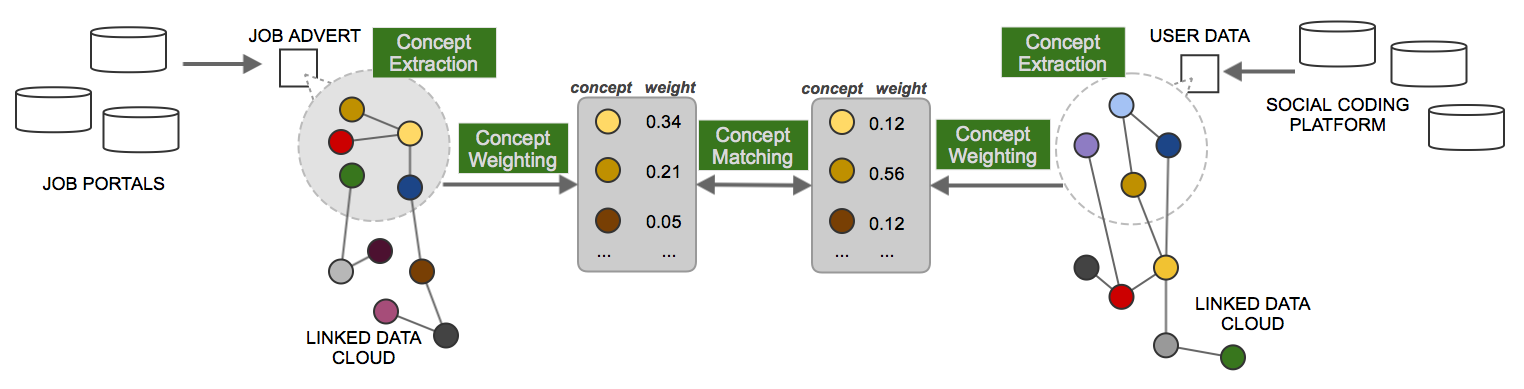
\includegraphics[scale=0.32]{../figs/pipeline.png}
\caption{Overview of our pipeline}
\label{fig:pipeline}
\end{figure*}

In order to find potential employers,
developers search for job openings in various online job portals and compare
their desires, experiences and activities with the described position. This is a
cumbersome process as many job advertisements are lengthy, mentioning a plethora
of programming languages, libraries and techniques that the perfect candidate
should be familiar with. Moreover, each of these items is usually conditioned
on the number of years of experience or the level of expertise and may fall into
the ``required'' or ``preferred'' skill category. Over the years, job
advertisements have asked for a larger number of skills from prospective
employees. This has led to a situation where a developer matching half of the
described requirements may actually be a very well qualified candidate for the
advertised position. In such cases having insights into how well other potential
candidates fit the position may help the developer to judge whether to apply or
not. Another complicating factor is the fact that job advertisements' writing
style may be influenced by the numerous people involved in the creation of a job
profile (managers, developers, HR personnel, etc.). Here a ``semantic gap'' may
exist between search terms a developer is using to find suitable advertisements
in job portals and the terms that actually appear in an advertisement.

Business-oriented social networks, such as
LinkedIn\footnote{\url{https://www.linkedin.com/}}, are using recommender engines
to \emph{push} job advertisements to their users (in addition to the traditional
\emph{pull}-based model where users are actively searching among the available
advertisements). Recommender algorithms determine the \emph{similarity} between
pairs of user and advertisement profiles and recommend the job to the user if
the similarity is high. While this process moves the burden of determining the
degree of matching away from the user, it is limited in its abilities due to the
lack of detailed user profile data as statements such as ``Experienced Java
developer'' or ``Embedded Software Engineer'' contain relatively little
information.

In the recent years, social coding platforms have become an important tool for
developers to become visible in the developer community~\cite{Capil13}.
Developers use sites such as GitHub and BitBucket to showcase their work in the
hope that this will help them in the hiring process by potential
employers~\cite{dabbish2012social}. However, judging the qualification of an
applicant based on his or her GitHub profile is equally
challenging~\cite{Singer:2013:MAS:2441776.2441791}. GitHub provides several
user-based summary statistics such as \emph{Contributions in the last year},
\emph{Number of forked projects}, \emph{Number of followers}, however, the
usefulness of this information is very limited, as neither does it offer
immediate insights into the developer's programming abilities nor does it
highlight the particular languages or tool chains the developer knows.

%We conclude that considering the vast amounts of job advertisements in the IT
%sector (as well as the large number of developers), finding a job advertisement
%that is a good match with one's own abilities and desires is currently an
%inefficient process and likewise, determining how well an applicant from a group
%of applicants matches the position based on available GitHub user data is
%cumbersome and time-consuming. At the same time though, GitHub user data
%provides detailed insights that are not possible to be gained from other social
%Web sources.
%

To address the process shortcomings we identified above, we propose a pipeline
that \emph{automatically} mines GitHub user profiles and job advertisements for
relevant information. We employ an approach that ``translates'' both the
developer profile and the advertisement into the Linked Open Data
(LOD)~\cite{bizer2009linked} space, where we can exploit the background
information available in the LOD cloud to bridge the semantic gap mentioned
earlier. Additionally, this setup allows us to (partially) rely on well-tested
algorithms and toolkits, while it provides a natural mechanism to determine the
similarity between a natural language job advertisement and a developer's GitHub
profile.

%In the following section we describe our proof-of-concept and provide an
%overview of the challenges that need to be overcome.

\section{Approach}

The general overview of our pipeline is shown in Figure~\ref{fig:pipeline}.
The three main components are:

\begin{itemize}

  \item \textbf{Extraction} of concepts from job advertisements and social
    coding user data.

  \item \textbf{Weighting} of concepts in such a way that more important
    concepts receive higher weights.

  \item \textbf{Matching} of the two (job and coding profile-based) concept
    vectors.

\end{itemize}

\subsection{Concept Extraction Overview}

%On the left-hand side in Figure~\ref{fig:pipeline}, we take as input a job
%advertisement in natural language text and extract the entities (or concepts)
%that appear in it.

\subsubsection{The DBPedia Ontology}
Our approach is based on two techniques from natural language processing namely,
\emph{named entity recognition} (NER) in combination with \emph{named entity
disambiguation} (NED). Given an unstructured text (e.g. a job advertisement) NER determines which words or phrases in the text refer to an
entity, which can be any real-world entity. NED
determines which concrete entity a particular word or phrase refers to.  The
combination of both techniques have been shown~\cite{aggarwal2012mining} to be a
powerful mechanism to turn natural language text into a structured representation
that machines can reason about.

%not the right place, but latex is pretty unwilling to render where I want this figure to be rendered
\begin{figure*}[!htb]
\centering
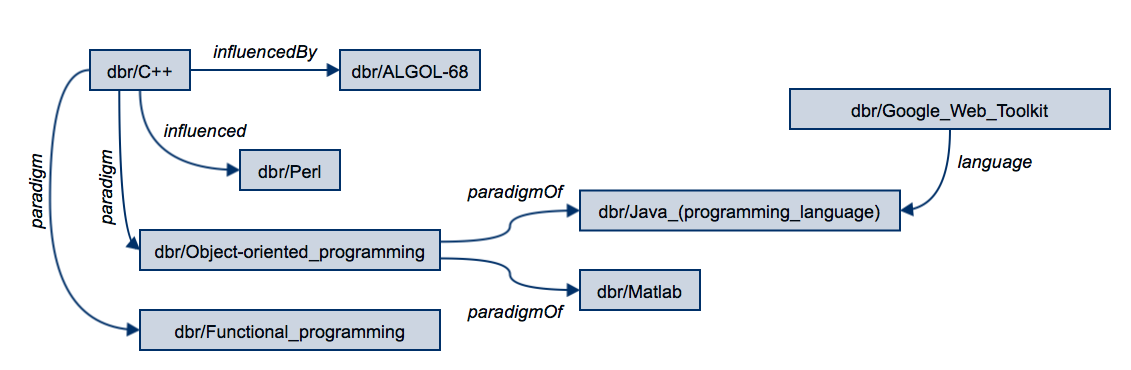
\includegraphics[scale=0.3]{../figs/dbpedia-example-graph.png}
\caption{An excerpt of DBPedia's graph structure. Each node is a concept, the properties between two concepts are captured in the form of a labelled edge.}
\label{fig:dbpedia-example}
\end{figure*}

We rely on DBPedia Spotlight,\footnote{\url{http://dbpedia-spotlight.github.io/}}
one of the most commonly used open-source annotation toolkits for natural
language text, as a concrete implementation of concept extraction. The
large-scale DBpedia ontology~\cite{mendes2011dbpedia} behind the DBPedia Spotlight service is
automatically derived from Wikipedia and (based on the English Wikipedia edition),
currently contains more than 4.5 million entities (``things'') and nearly 600
million links between them. Wikipedia (and thus DBPedia) contain entries
covering most if not all programming languages, important programming
frameworks and libraries, as well as many computer science concepts. We thus
consider it a suitable ontology to use for our specific use case.

\subsubsection{A Concrete Example}
Consider the following excerpt from one of the job
advertisements in our data set and its corresponding automatically derived Named
Entity annotations. Shown in bold are all phrases that were recognized as
referring to entities (or concepts). The annotations relevant to our scenario
are shown in blue, while non-relevant entities are shown in red.

\vspace{1em}
{\small

\noindent The \textbf{successful} \annotateG{Successful\_(song)}\\
\textbf{candidates} \annotateG{Candidate} \\
will have \textbf{experience} \annotateG{Experience}\\
of \textbf{OOP} \annotate{Object-oriented\_programming}\\
in at least one of \textbf{PHP} \annotate{PHP}\\
(or another comparable,\\
dynamic language), \annotate{Dynamic\_programming\_language}\\
\textbf{Java} \annotate{Java\_(programming\_language)}\\
(ideally with \textbf{GWT}) \annotate{Google\_Web\_Toolkit}\\
or \textbf{C++} \annotate{C++}\\
(ideally with \textbf{Win32}). \annotate{Windows\_API}\\
They will also be well versed in\\
\textbf{Test Driven Development} \annotate{Test-driven\_development}\\
and advanced practices of\\
{\footnotesize\textbf{Object Oriented Programming}} \annotate{Object-oriented\_programming} \\
such as Design Patterns and \textbf{Refactoring}. \annotateG{Martin\_Fowler}}\\

The
phrases (the so-called \emph{surface form} of an entity) are not simply matched
against a list of entity names, instead they are disambiguated based on the
context a word or phrase appears in. For instance, \emph{Java}is recognized as
the programming language concept (instead of the island, the coffee type or
another one of the more than 30 different entities that have the surface form
\emph{Java}). Each entity is uniquely identified as a particular LOD concept.
%which in the case of DBPedia Spotlight is prefixed by
%\texttt{http://dbpedia.org/resource/} (for brevity, we replaced this prefix with
%\texttt{dbr} above).
Concepts are linked to each other through different types
of properties, thus forming a densely connected graph structure.
Figure~\ref{fig:dbpedia-example} contains a small excerpt of this graph; even
though C++ and the Java programming language are not directly linked, we can
determine some degree of relatedness by a walk across the graph or by considering the textual similarity between each entity's description~\cite{gabrilovich2007computing} (similarly, we
can observe a lower relatedness degree between C++ and the GWT, as the distance
between the two concepts is larger). Since in our particular use
case we are mostly interested in concepts related to information technology, we
restrict the annotations to concepts that have the type \emph{computer} or
\emph{internet}.

\subsection{Developer Profile Extraction}

While the annotation of the job advertisements is straight-forward (as just shown in the example), annotating a developer's GitHub data with concepts from the same ontology (to allow a simple
matching strategy) is more challenging. While programming language
identification can largely be considered a solved problem, more fine-grained
information such as the libraries used by a particular project often require
language-specific solutions (e.g. Maven projects requires the parsing of
\textsf{pom.xml} files). Furthermore, identifying the degree of familiarity a
developer has with particular concepts (e.g. WebSocket programming, the TCP
protocol, Bloom filters) requires deep parsing and semantic tagging of the
developer's source code contributions; parsing at scale requires vast computing
resources while concept extraction from source code is neither precise nor complete~\cite{Kuhn07}.

We advocate that README (and in general, documentation) files in repositories in
the developer's profile are a good proxy for the developer's familiarity with
certain programming concepts, languages and toolkits. A typical README file
contains information about what the software can do, description of technologies
used in it, steps on how to recreate development environments and in general a
wealth of information that the developers should be familiar with if they own a
repository. Since such READMEs are in natural language form, we can use exactly
the same process as for the job advertisements, only instead of extracting the
concepts of a single piece of text, we process all README files contained in all
projects the developer is associated with. 
 %Here, association can either mean a repository the developer created or forked.

\subsection{Concept weighting}

The extracted concepts from job descriptions and GitHub developer profiles are converted
to vectors: $\textit{job}_i=(w_{1,i}, w_{2,i}, ..., w_{n,i})$ and $\textit{dev}_j=(w_{1,j},
w_{2,j}, ..., w_{n,j})$. Each dimension corresponds to one DBPedia concept and
if a concept $c_s$ is found in the job advertisement (or developer profile), the
corresponding weight $w_{s}$ is set to a value above zero. Since these vectors
are extremely sparse, in the future we will also investigate the use of semantic relatedness measures on the DBPedia data to ``switch on'' related concepts that are not explicitly mentioned in the
advertisement or developer profile.
%How to exactly set the weights is the task
%of the concept weighting component discussed next.

Not all concepts extracted from an advertisement or developer profile are equally important. We use a basic concept weighting scheme commonly employed in information retrieval: TF.IDF~\cite{baeza1999modern} which gives a low weight to concepts that appear in many documents (as those are not very informative) while at the same time benefiting concepts which occur rarely across the entire corpus of documents, but often within particular documents. These weights are computed separately for the corpus of job advertisements and the corpus of developer profiles. 

%Additionally, we enrich the concept vectors by adding for each found concepts up to $t$ semantically related concepts based on a particular relatedness measure \claudia{is this through the ``random walks''? I do not understand, please explain a bit more}.

\subsection{Concept matching}

The vector space model~\cite{baeza1999modern} provides a natural mechanism to determine the similarity
between the devised job and developer profile vectors, namely the cosine of the
angle between the two vectors (the so-called cosine similarity), which is
bounded to a value in $[0,1]$ where a larger score indicates higher similarity.
We can now for each job advertisement rank all developer profiles according to the similarity as well the other way round.

\section{Preliminary Results}

\paragraph{Job advertisements} 
We crawled job advertisements posted in early 2015 from the UK job portal  Indeed\footnote{\url{http://www.indeed.co.uk}}. Each search on Indeed returns up to $1,000$ search results (i.e. advertisements); we conducted five searches using the following search phrases: $\{\textit{software developer}, \textit{software architect}, \textit{software engineer},$ $\emph{computer science}, \emph{web developer}\}$ and thus retrieved $5,000$ advertisements in total. Of those more than $1,300$ advertisements were posted directly on the Indeed platform (instead of referring to an externally placed advertisment). We annotated them with DBPedica concepts as discussed before; the main results are shown in Table~\ref{tab:jobadverts}. Important for our work is the fact that on average ten IT concepts are mentioned in each advert. The ten most occurring concepts in this data set are shown in Table~\ref{tab:top10} (left column). 

\begin{table}
\centering
\begin{tabular}{lr}
\toprule
Number of job adverts								& $1,337$\\
Average number of words / advert 			& $284.7$\\
\midrule
Aveage number of entities / advert			& $84.1$\\
Average number of  distinct entities / advert	& $59.0$\\
\midrule
Average number of IT entities / advert	& $14.4$\\
Average number of distinct IT entities / advert& $9.7$\\
\midrule
Total number of distinct IT entities found	& 486\\
\bottomrule
\end{tabular}
\caption{Overview of our job advertisement data set.}
\label{tab:jobadverts}
\end{table}

\begin{table}
\centering
\footnotesize
\begin{tabular}{ll}
\toprule
\textbf{Job advertisements}	& \textbf{Developer profiles}\\
\midrule
Computer\_software (41.8\%) 			& Hypertext\_Transfer\_Protocol (78.0\%) \\
Application\_software (39.6\%)		& Scripting\_language (67.0\%) \\
Cascading\_Style\_Sheets (37.8\%)	& HTML (67.0\%) \\
Business (36.4\%)								& COM\_file (61.1\%)\\
JavaScript (34.5\%)							& Debian (60.5\%)\\
HTML (23.0\%)									& JavaScript (56.4\%) \\
Debian (19.2\%)								& Library\_computing (44.8\%) \\
PHP (18.9\%)									& Git\_(software) (29.2\%) \\
Computing\_platform (18.4\%)		& GNU\_Project (29.2\%) \\
.NET\_Framework (18.0\%)				& Wiki (27.5\%)\\
\bottomrule
\end{tabular}
\caption{Overview of the ten most often occurring IT concepts in our job advertisement and developer profile data sets. Shown in brackets is the percentage of documents (job advertisements / developer profiles) that contain the concept at least once.}
\label{tab:top10}
\end{table}

\paragraph{Developer profiles}

\begin{figure}
\vspace{-0.1cm}
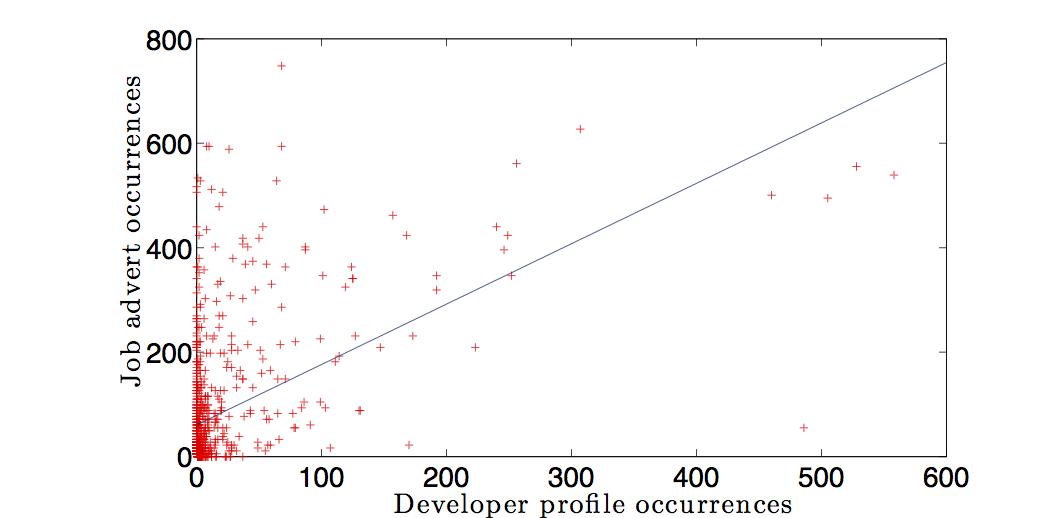
\includegraphics[scale=0.3]{../figs/entities-jobs-vs-devs.png}
\caption{Each marker represents one IT entities (851 in total) which represent the union of all concepts found in the job adverts and developer profile data sets. The scatter plot shows in how many developer profiles the entity appeared (at least once) vs. in how many job advertisements.}
\label{fig:scatterEntities}
\vspace{-0.5cm}
\end{figure}

We extracted the $1,000$ top committers from the GHTorrent~\cite{Gousi13} dataset. 863 of those users forked or created at least one project that contains a non-empty \texttt{REAdME.md} file, the remainder are either bots (63 users) or created/forked projects with only empty README.md files (70 users). Thus, overall for less than $10\%$ of human GitHub it is not possible to use README's as source of developer profile data. Each \texttt{README.md} is associated with one project. The main statistics of our developer data set are shown in Table~\ref{tab:developers}. Importantly on average for each developer we are able to extract $500$ IT entities across all the developer's README files. The $57$ distinct IT entities found on average per developer indicate the high level of detailed information we are able to extract. The right column of Table~\ref{tab:top10} shows the most often occurring IT entities across developers. In support of our envisioned application, we find substantial overlap between the entities extracted from job advertisements and the entities extracted from developer profiles as evident in Figure~\ref{fig:scatterEntities}; while some concepts appear either only among the developer profiles or among the job adverts, the majority of concepts appear at least once in both corpora. The linear correlation between the number of times a concept appears in developer profiles vs. job adverts is $r=0.49$ (fitted line in Figure~\ref{fig:scatterEntities}).

\begin{table}[htb]
\centering
\begin{tabular}{lr}
\toprule
Number of developers									& $863$\\
\midrule
Average number of project README files / developer	& $32.3$\\
Average number \emph{forked} project README files / developer	& $16.5$\\
Average number \emph{created} projet README files / developer & $15.7$\\
\midrule
Average number of words / README file		& $384.5$\\
Average number of non-code words / README file 	& $320.2$\\
\midrule
Average number of entities / README file 					& $52.3$\\
Average number of distinct entities / README file 					& $17.23$\\
\midrule
Average number of IT entities / README file				& $18.0$\\
Average number of distinct IT entities / README file				& $6.0$\\
\midrule
Average number of entities /developer						& $1447.3$\\
Average number of distinct entities / developer			& $291.3$\\
Average number of IT entities / developer			& $500.1$\\
Average number of distinct IT entities / developer		& $78.1$\\
\midrule
Total number of distinct IT entities found	& $764$\\
\bottomrule
\end{tabular}
\caption{Overview of our developer profile data set.}
\label{tab:developers}
\end{table}


\paragraph{Matching developer and job profiles}

Lastly, for every pair of job advert and developer profile vector we computed their similarity. A manual investigation of the developer rankings produced for 25 adverts showed reasonable results though it also became clear that additional GitHub signals (number of lines of code, coding style and quality, etc.) are required as extensive README files do not always equate to extensive coding. Similarly, more fine-grained distinctions for forked and created projects are likely to aid the results.


\section{Related Work}

Profiling developers using trace data is an active field of research. Developer
profiles have been built, among others, for building project-specific expertise
knowledge bases~\cite{Mocku02}, identify developers with similar
expertise~\cite{Schuler08}, measure develop productivity~\cite{Gousi08},
and recommending developers for specific tasks~\cite{ying14} (e.g. bug
resolution~\cite{Anvik06}). However, to the best of our knowledge, no work
extracted developer profiles for matching with job advertisements.

In reference~\cite{Capil13}, Capiluppi et al. described a process (and its
pitfalls) for assessing technical candidates using data, among others, from
social coding sites. Marlow et al.~\cite{Marlow:2013:ATS:2441776.2441794}
investigated how more detailed, publicly accessible signals about a developer's
activities on GitHub are used by employers in the recruitment process. In an
interview-based study with several IT employers (active in the open-source
community) they identified four main insights that employers can \emph{reliably}
gain from a study of developer GitHub profiles: (1) Shared open source values,
(2) Community acceptance of work \& contribution quality, (3) Project management
skills, and (4) Passion for coding. Though again, the limiting factor in this
setup is the time required to manually inspect each developer's profile.

\section{Conclusions}

The availability of data from social coding sites enables the automated
extraction of developer profiles for the purposes of matching them with job
advertisements. We proposed a pipeline to do this matching automatically.  Our
key insights are( i) the approximation of the developers' actual programming
knowledge through README files in their profile repositories, and, (ii) the use of a
large scale ontology to convert both job advertisements and developer profiles
to vector objects featuring a common vocabulary. We obtained interesting
insights such as the substantial overlap in covered concepts between adverts and README files and the abundance of IT concepts in the latter, which leads us to believe that our approach is a
promising start. In the future, we plan to augment developer profiles through extracting fine-grained information from the source code and build files for
their repositories.

\bibliographystyle{IEEEtran}
\bibliography{dev-profiles}


\end{document}
